\section{ОГЛЯД ПІДХОДІВ ДО РЕПРЕЗЕНТАЦІЇ СТРУКТУРИ РЕЧЕННЯ}
Природню мову можна розглядати як з точки зору статистики, уявляючи слова як унітарні вектори,
з якими можна робити різні трансформації, як-от додавання контексту чи інших видів
інформації, для того, щоб прогнозувати певні послідовності. Так і уявляти мову як
набір об'єктів або токенів, які описують явища, які ми, люди, розуміємо. Наприклад,
іменники, дієслова, дієслівні групи та іменні групи, що в українській мові
може трактуватися як іменникове (субстантивне) словосполучення –-- словосполучення 
з іменником у ролі головного слова~\cite{bib3}. Та намагатися зрозуміти як
ці об'єкти взаємодіють одне з одним в граматичному сенсі.

\subsection{Конституентний парсинг}
Якщо розглядати мову тільки з точки зору статистистики, тобто як послідовності N-грам, токенів
чи символів, які є унітарними векторами, ми можемо створювати моделі мови, тобто трансформери,
або виводити інші приховані властивості, такі як частини мови, тощо. Але в природній мові слова
можуть мати значення, яке виходить за межі їхньої символьної репрезентації. Адже природня
мова --- це не просто набір токенів. Речення підкоряються певним граматичним правилам і мають
контекст, у якому вони вживаються. Цей контекст не міститься напряму в реченні, але ми, люди,
інтуїтивно його розуміємо, базуючись на нашому попередньому досвіді, природних явищах, поведінкових
шаблонах, тощо. Від цього контексту напряму залежить те, як ми інтерпритуємо те, чи інше речення.

\begin{figure}[H]
  \begin{center}
    \noindent $S \rightarrow T \mid U$ \\
    \noindent $T \rightarrow VaT \mid VaV \mid TaV$ \\
    \noindent $U \rightarrow VbU \mid VbV \mid UbV$ \\
    \noindent $V \rightarrow aVbV \mid bVaV \mid \varepsilon$ \\
  \end{center}
  \caption{Контекстно-вільна граматика}
  \label{text:context_free_grammar}
\end{figure}

Із достатнім набором даних можливо натренувати модель, яка буде розуміти певні граматичні
закономірності, але якщо розширити цей набір даних правилами і тонкощами мови --- це значно підвищить релевантність цієї моделі.

Контекстно-вільна граматика (КВГ) --- це набір правил, які визначають те, як потрібно класифікувати,
групувати та розміщувати мовні токени в ієрархічні граматичні структури. Символи, що
відповідають за слова у мові, називають термінальними символами. Вони також є і кінцевими
токенами, які можна зустріти у наборах даних. Набір правил, який оголошує термінальні
символи називають лексиконом~\cite{bib5}. Розглянувши приклад
\texttt{Іменник~$\rightarrow$~кіт~$\mid$~риба~$\mid$~курка~$\mid$~дорога}, можна зрозуміти
що термінальними символами є \texttt{кіт, риба, курка, дорога}. У більш узагальненому
вигляді контекстно-вільна граматика зображена на рисунку~\ref{text:context_free_grammar}.

Якщо створити правильний набір правил, ми можемо використовувати КВГ для того, щоб парсити
існуючі тексти, або навіть генерувати нові, такі, що задовольняють правилам нашої граматики.

Оголосивши граматику~\ref{text:cfg_uk}, та просто застосовуючи її правила,
ми можемо розібрати речення \texttt{Дідо Богдан був тоді в італійському полоні}.
При проходженні правил, що містять тільки термінальні символи, ми отримаємо
\texttt{[{\footnotesize Noun}Дідо] [{\footnotesize Noun}Богдан] 
[{\footnotesize Verb}був] [{\footnotesize Adverb}тоді]
[{\footnotesize Proposition}в] [{\footnotesize Adjective}італійському]
[{\footnotesize Noun}полоні}]. 

\begin{figure}[H]
  \begin{center}
    \noindent Noun $\rightarrow$ Дідо $\mid$ Богдан $\mid$ полоні $\mid$ ... \\
    \noindent Verb $\rightarrow$ був $\mid$ ...\\
    \noindent Adjective $\rightarrow$ італійському $\mid$ ... \\
    \noindent Adverb $\rightarrow$ тоді $\mid$ ... \\
    \noindent Proposition $\rightarrow$ в $\mid$ ... \\
    \noindent Nominal $\rightarrow$ Noun $\mid$ Nominal Noun \\
  \end{center}
  \caption{Задана КВГ}
  \label{text:cfg_uk}
\end{figure}

Використавши останнє правило для Nominal, ми об'єднаємо
2 іменника в одну групу 
\texttt{[{\footnotesize Nominal}[{\footnotesize Noun}Дідо][{\footnotesize Noun}Богдан]]
[{\footnotesize Verb}був] [{\footnotesize Adverb}тоді] [{\footnotesize Proposition}в]
[{\footnotesize Adjective}італійському] [{\footnotesize Noun}полоні}].

Таким чином ми можемо отримати структуру, схожу на дерево. Дійсно, нотація з використанням
квадратних дужок є лише скороченною формою запису
абстрактного дерева розбору (parse tree), рисунок~\ref{text:parse_tree}.
Отже, ми можемо зробити висновок, що абстрактне дерево розбору є результатом слідування
правил із заданої контекстно-вільної граматики. 

Такі правила ми можемо використовувати не
тільки для того, щоб парсити існуючі тексти, а й щоб генерувати нові. Наприклад, якщо
просто вибирати випадкові термінальні символи, дуже рідко можна отримати якесь осмисленне
речення, але додавши до такого підходу ймовірнісні методи, можна отримати речення, які
несуть в собі більше сенсу.

\begin{figure}[H]
  \centering
  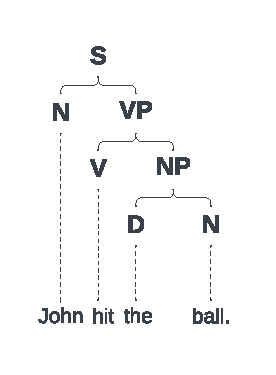
\includegraphics[width=0.4\textwidth]{parse_tree.pdf} 
  \caption{Приклад дерева розбору}
  \label{text:parse_tree}
\end{figure}

Використовуючи тільки КВГ, ми не вказуємо яким конкретно чином ми повинні генерувати
абстрактне дерево розбору. Для деяких реченнь, змінивши порядок в яких застосовуються ці
правила, ми отримаємо різні дерева розбору. Тому нам потрібен алгоритм, який буде 
використовувати КВГ, при цьому на виході повертати найбільш коректне дерево розбору.
Ці неоднозначності умовно можна поділити на 2 категорії:
\begin{enumerate}
    \item Вкладення: коли даний конституент може бути вкладеним до дерева розбору
    більше, ніж в одному місці.
    \item Координація: коли різні набори фраз можуть буди розділені сполучником.
    Наприклад ``сіра парасолька та трава''. Де не зрозуміло, ``сіра'' відноситься
    тільки до парасольки, чи також і до трави.
\end{enumerate}

Процес, який дозволяє обрати коректний варіант із декількох варіантів розбору називаєтся
прибиранням синтаксичних неоднозначностей (syntactic disambiguation). Найбільш
популярним алгоритмом динамічного програмування, який вирішує цю проблему є
алгоритм Кока — Янгера — Касамі (CKY)~\cite{bib6}. Для того, щоб
використовувати цей алгоритм, потрібно щоб КВГ була представлена у вигляді
нормальної форми Чомскі~\cite{bib7}, тобто граматика складалася тільки
з двох нетермінальних символів, або з одного термінального символа.

\subsection{Парсинг залежностей}
У конституентного парсингу є два фатальні недоліки, які не дозволяють
моделювати важливі структурні та лексичні залежності:
\begin{enumerate}
    \item Припущення про незалежність: такий метод спирається на статистичні
    вірогідності, які не є точними на сто відсотків, що може призводити до
    неправильного моделювання залежностей.
    \item При моделюванні не враховуються деякі синтаксичні факти щодо певних слів,
    що може призводити до підкатегоризації слів, що мають однакове значення,
    або може втрачатися інформація про об'єднання прийменника та іменника
    в одну групу.
\end{enumerate}

Конституентний парсинг --- це не єдиний спосіб парсингу інформації у реченні.
Іншим способом є парсинг залежностей (dependency parsing). Кожне слово у
реченні можна логічно з'єднати з іншим словом, від якого вого залежить,
при цьому вказавши тип зв'язку між цими двома словами. Таким чином, речення
постане у вигляді дерева, де вузли будуть словами, а грані --- залежностями.
У такому формалізмі, синтаксична структура речення представлена
виключно з точки зору слів та набору направлених бінарних граматичних відношеннь,
які є між цими словами. Таким чином результатом парсингу уже є не дерево розбору,
а дерево залежностей, рисунок~\ref{img:dependency_tree}.
\begin{figure}[ht]
  \begin{center}
    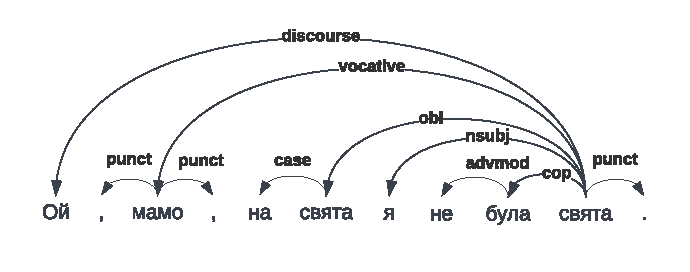
\includegraphics[width=\textwidth]{dependency_tree.pdf}
  \end{center}
  \caption{Дерево залежностей}
  \label{img:dependency_tree}
\end{figure}

Ці залежності зазвичай ілюструють як направлені дуги з мітками, від кореневого
елементу, до тих, від якого він залежить.

Використовуючи такий підхід, нам більше не потрібно хвилюватися про
порядок слів у реченні, на відміну від контекстно-вільних граматик, де ми
ітерували по реченню зліва направо, у прямому порядку слів.

Дуже добре парсинг залежностей проявляє себе у текстах з прямою мовою
де дуже важко розставити зв'язки між членами речення.

Такі структури залежностей представлені у вигляді направлених графів та
повинні задовольняти наступним умовам:
\begin{enumerate}
    \item У реченні є тільки одна коренева вершина, у якої немає вхідних зв'язків.
    \item Кожна вершина повинна мати тільки один вихідний зв'язок, за
    винятком кореневої вершини.
    \item Є тільки один шлях від кореневої вершини, до кожного
    вузла у реченні. Тобто такий направлений граф є деревом.
\end{enumerate}

Існують два основні підходи до створення алгоритмів, що генерують дерева
залежностей із вхідних даних:
\begin{enumerate}
    \item Транзиційні підходи (Transition-based approaches), до яких відносять парсери
    Shift-reduce.
    \item Алгоритми на основі графів та виділенню кістякових дерев.
\end{enumerate}

Деякі алгоритми є проективними, тобто зв'язки між вузлами не можуть пересікатися, як
це зображено на рисунку~\ref{img:dependency_tree}. Більшість реченнь у мові
влаштована саме таким чином. Але є й речення, у яких грані графа перетинаються. Тому це
потрібно враховувати при обробці відповідних наборів даних.

Коли ми говоримо про транзиційні підходи, найчастіше маються на увазі
парсери, які побудовані на основі програмного стеку. Такі парсери структурно можна
розділити на дві функції, які вони виконують. Перша --- це машина побудована на стеку,
яка кладе слова речення на верхівку цього стеку. Друга --- безпосередньо
сам парсер, або натренована нейронна мережа, яка вирішує яким чином потрібно
розставляти зв'язки між термінальними членами речення. Саме цей парсер і будує
граф, розставляючи ці зв'язки, у яких є тільки два напрями: вправо і вліво.
Він бере два останні елементи на стеку та встановлює між ними відношення~\cite{bib8}.
Такі парсери будують на основі тренованих нейронних мереж, які
стають класифікаторами токенів. Найбільшою вибіркою даних для навчання цих класифікаторів
є корпуси текстів Universal Dependencies.

\subsection*{Висновки до розділу \arabic{section}}
\addcontentsline{toc}{subsection}{Висновки до розділу \arabic{section}}
У цьому розділі було розглянуто найпопулярніші методи для репрезентації структури
речення, освітлено їхні недоліки та переваги. Було описано метод парсингу
залежностей у контексті теми цієї роботи та корпусу текстів Universal
Dependencies. Досліджено існуючі алгоритми реалізації цих методів та описано
приклади розбору заданих формальних граматик.